\documentclass{standalone}
\begin{document}
\subsection{Prediction of Response}

In order to measure the accuracy of the classification for each class (Class 0 for complete response and Class 1 for moderate response), I used different metrics: 
\subsubsection{Precision}
Intuitively, it is the ability of the classifier not to label as positive a sample that is negative: 
\begin{equation*}
    Precision = \frac{tp}{tp + fp}
\end{equation*}

\subsubsection{Recall}
Intuitively, it is the ability of the classifier is the ability of the classifier to find all the positive samples: 
\begin{equation*}
    Precision = \frac{tp}{tp + fn}
\end{equation*}

\subsubsection{F1-Score}
It is the harmonic mean of the precision and recall: 
\begin{equation*}
    F1\mathtt{-}Score = 2 \cdot \frac{precision \cdot recall}{precision + recall}
\end{equation*}
\\

where $tp$ is the number of true positives and $fn$ the number of false negatives.
\\
\\
The results are shown in Table \ref{tab:classreport}, where for each class you get the relative score.
The \textit{support} column indicates the population for that class.
As you can see, for Class 0 the scores are lower compared to Class 1 but also the \textit{support} is lower since the cases of a complete response were less compare to the number of case of a moderate one.
The sum of the \textit{support} is 32 corresponding to the number of patients involved into the analysis.




\begin{table}[ht]
	\centering
	\begin{tabular}{ccccc}
		\toprule
		  & \textbf{Precision}  & \textbf{Recall} & \textbf{F1-Score} & \textbf{Support}\\
	    \midrule
		\textbf{Class 0} &  0.71 &  0.77 &  0.74 &  13\\
	    \midrule
		\textbf{Class 1} &  0.83 &  0.79 &  0.81 &  19\\
		\bottomrule
	\end{tabular}
	\caption{Classification report}
	\label{tab:classreport}
\end{table}

\newpage
I also computed the confusion matrix (or error matrix), in Figure \ref{confmatrix}, to evaluate the accuracy of the classification.
Each row of the matrix represents the instances in an actual class while each column represents the instances in a predicted class.
As you can see from the confusion matrix, on the diagonal you have the number of well-classified instances while on the anti-diagonal the wrong-classified ones.
For Class 0, so for a complete response, the well-classified instances are 10 over a total of 13, thus the wrong-classified ones are 3.
For Class 1, so for a moderate response, the well-classified instances are 15 over a total of 19, thus the wrong-classified ones are 4.


\begin{figure}[htp]

    \centering
    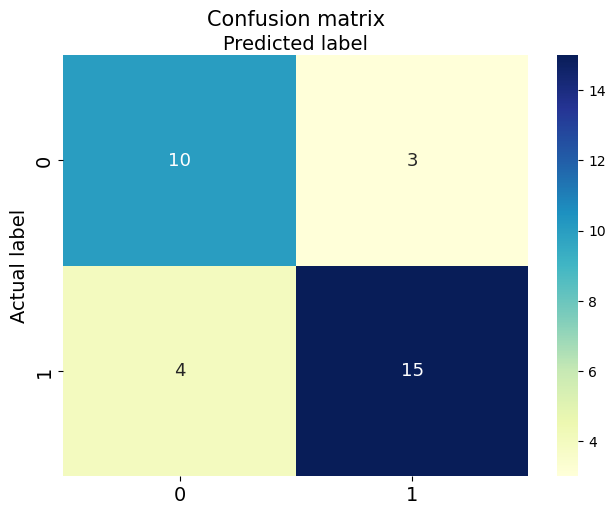
\includegraphics[width=0.75\textwidth]{../images/confmatrix.png}

    \caption{Confusion Matrix. The rows of the matrix represents the instances in an actual class while each column represents the instances in a predicted class. Class 0 means a complete response while Class 1 a moderate one. }
    \label{confmatrix}
    
\end{figure}


The diagnostic ability of the classifier was also measured by the Receiver Operating Characteristic curve, or ROC curve.
The ROC curve is created by plotting the true positive rate (TPR) against the false positive rate (FPR).
By analyzing the ROC curves, the ability of the classifier to discern, for example, between a set A and B of population, is assessed, calculating the area under the ROC curve: Area Under Curve, (AUC). 
The AUC value, between 0 and 1, is equivalent to the probability that a classifier will rank a randomly chosen positive instance higher than a randomly chosen negative one.
The ROC curves pass through the points (0,0) and (1,1), (0,1) and (1,1) represent two limit curves:
\begin{itemize}
    \item The first cuts the graph at $45$ degrees, representing the case of the random classifier ("no benefit" line), with the AUC equal to 0.5.
    \item The second curve is represented by the segment that from the origin rises to the point (0,1) and by the one that connects the point (0,1) to (1,1), having the AUC equal to 1, meaning a perfect classifier.
\end{itemize}
In Figure \ref{ROC}, the ROC curve for the classifier is shown.
As you can see, the AUC both for classes is 0.82, greater than 0.5 which would correspond to a random classifier, that would give no benefit. 
I computed the average curve for Class 0 and Class 1, both considering class imbalance (micro-average) and not considering it, so giving the same weight to the classes (macro-average). 
Also for this case the AUC is greater than 0.5, meaning that the classifier prediction gives more benefit than a random one.

\begin{figure}[htp]

    \centering
    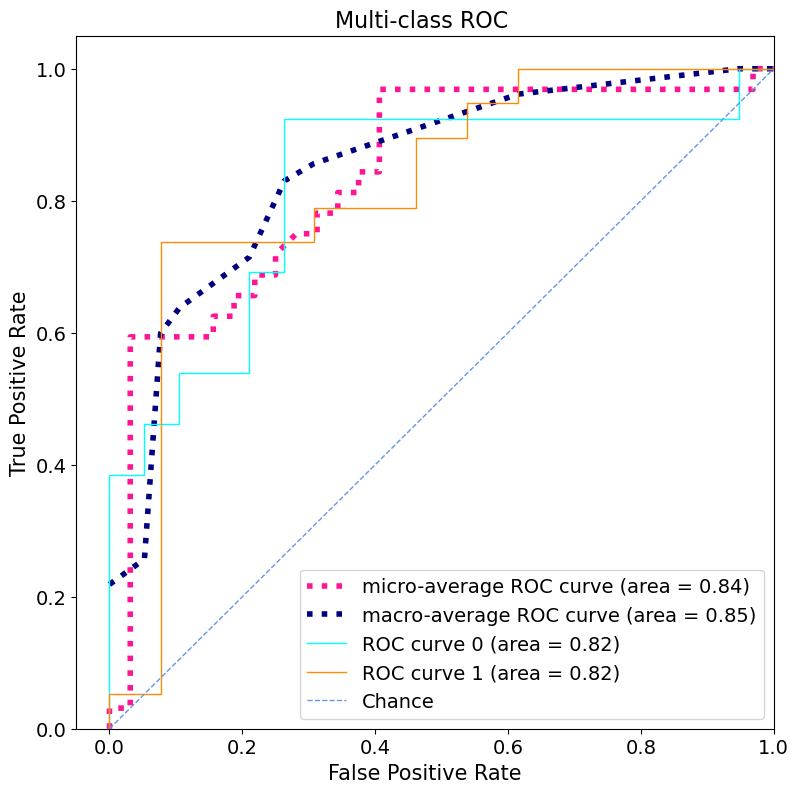
\includegraphics[width=0.75\textwidth]{../images/ROC.png}

    \caption{Receiver Operating Characteristic curve, or ROC curve.}
    \label{ROC}
    
\end{figure}

\end{document}